\documentclass[11pt]{article}
\usepackage[margin=0.8in]{geometry}
\usepackage[T1]{fontenc}
\usepackage{mathptmx}
\usepackage{amsmath,amssymb,booktabs,array,longtable}
\usepackage{graphicx}
\graphicspath{{figures/}}
\usepackage{caption}
\usepackage{hyperref}
\usepackage{enumitem}
\setlist{nosep}
\usepackage{xcolor}

\begin{document}

\begin{center}
{\large\textbf{Additional Task}}\\
{\large\textbf{Multi-Layer Perceptron Learning Algorithm for the XOR Gate}}
\end{center}

\section*{Objective}
A small multi-layer network was built for the XOR gate: 2 inputs, 2 hidden neurons with step
activation, and 1 output neuron with step activation. All three neurons were trained using the
plain perceptron delta rule, the same rule used for the single layer perceptron earlier in this
report, with no backpropagation. The weights and bias were printed after every single update, the
decision boundary was plotted after every update, and the pattern that stops the network from
converging was studied.

\section*{Training Log}
{\scriptsize
\begin{verbatim}
Epoch 1, sample [0 0], target 0, pred 1 ->
    W_hidden=[[-0.025, 0.09], [0.046, 0.02]], b_hidden=[-0.169, -0.169],
    W_out=[-0.088  0.073], b_out=-0.080
Epoch 1, sample [0 1], target 1, pred 0 ->
    W_hidden=[[-0.025, 0.19], [0.046, 0.12]], b_hidden=[-0.069, -0.069],
    W_out=[-0.088  0.073], b_out=0.020
Epoch 1, sample [1 1], target 0, pred 1 ->
    W_hidden=[[-0.125, 0.09], [-0.054, 0.02]], b_hidden=[-0.169, -0.169],
    W_out=[-0.188 -0.027], b_out=-0.080
  epoch 1 misclassified: 3

Epoch 2, sample [0 1], target 1, pred 0 ->
    W_hidden=[[-0.125, 0.19], [-0.054, 0.12]], b_hidden=[-0.069, -0.069],
    W_out=[-0.188 -0.027], b_out=0.020
Epoch 2, sample [1 1], target 0, pred 1 ->
    W_hidden=[[-0.225, 0.09], [-0.154, 0.02]], b_hidden=[-0.169, -0.169],
    W_out=[-0.188 -0.027], b_out=-0.080
  epoch 2 misclassified: 2

Epoch 3, sample [0 1], target 1, pred 0 ->
    W_hidden=[[-0.225, 0.19], [-0.154, 0.12]], b_hidden=[-0.069, -0.069],
    W_out=[-0.188 -0.027], b_out=0.020
Epoch 3, sample [1 1], target 0, pred 1 ->
    W_hidden=[[-0.325, 0.09], [-0.254, 0.02]], b_hidden=[-0.169, -0.169],
    W_out=[-0.188 -0.027], b_out=-0.080
  epoch 3 misclassified: 2

...

Epoch 30, sample [0 1], target 1, pred 0 ->
    W_hidden=[[-2.925, 0.19], [-2.854, 0.12]], b_hidden=[-0.069, -0.069],
    W_out=[-0.188 -0.027], b_out=0.020
Epoch 30, sample [1 1], target 0, pred 1 ->
    W_hidden=[[-3.025, 0.09], [-2.954, 0.02]], b_hidden=[-0.169, -0.169],
    W_out=[-0.188 -0.027], b_out=-0.080
  epoch 30 misclassified: 2

Misclassified samples per epoch:
[3, 2, 2, 2, 2, 2, 2, 2, 2, 2, 2, 2, 2, 2, 2, 2, 2, 2, 2, 2, 2, 2, 2, 2, 2, 2, 2, 2, 2, 2]
\end{verbatim}
}

\section*{Decision Boundary Plots}

\begin{figure}[h!]
\centering
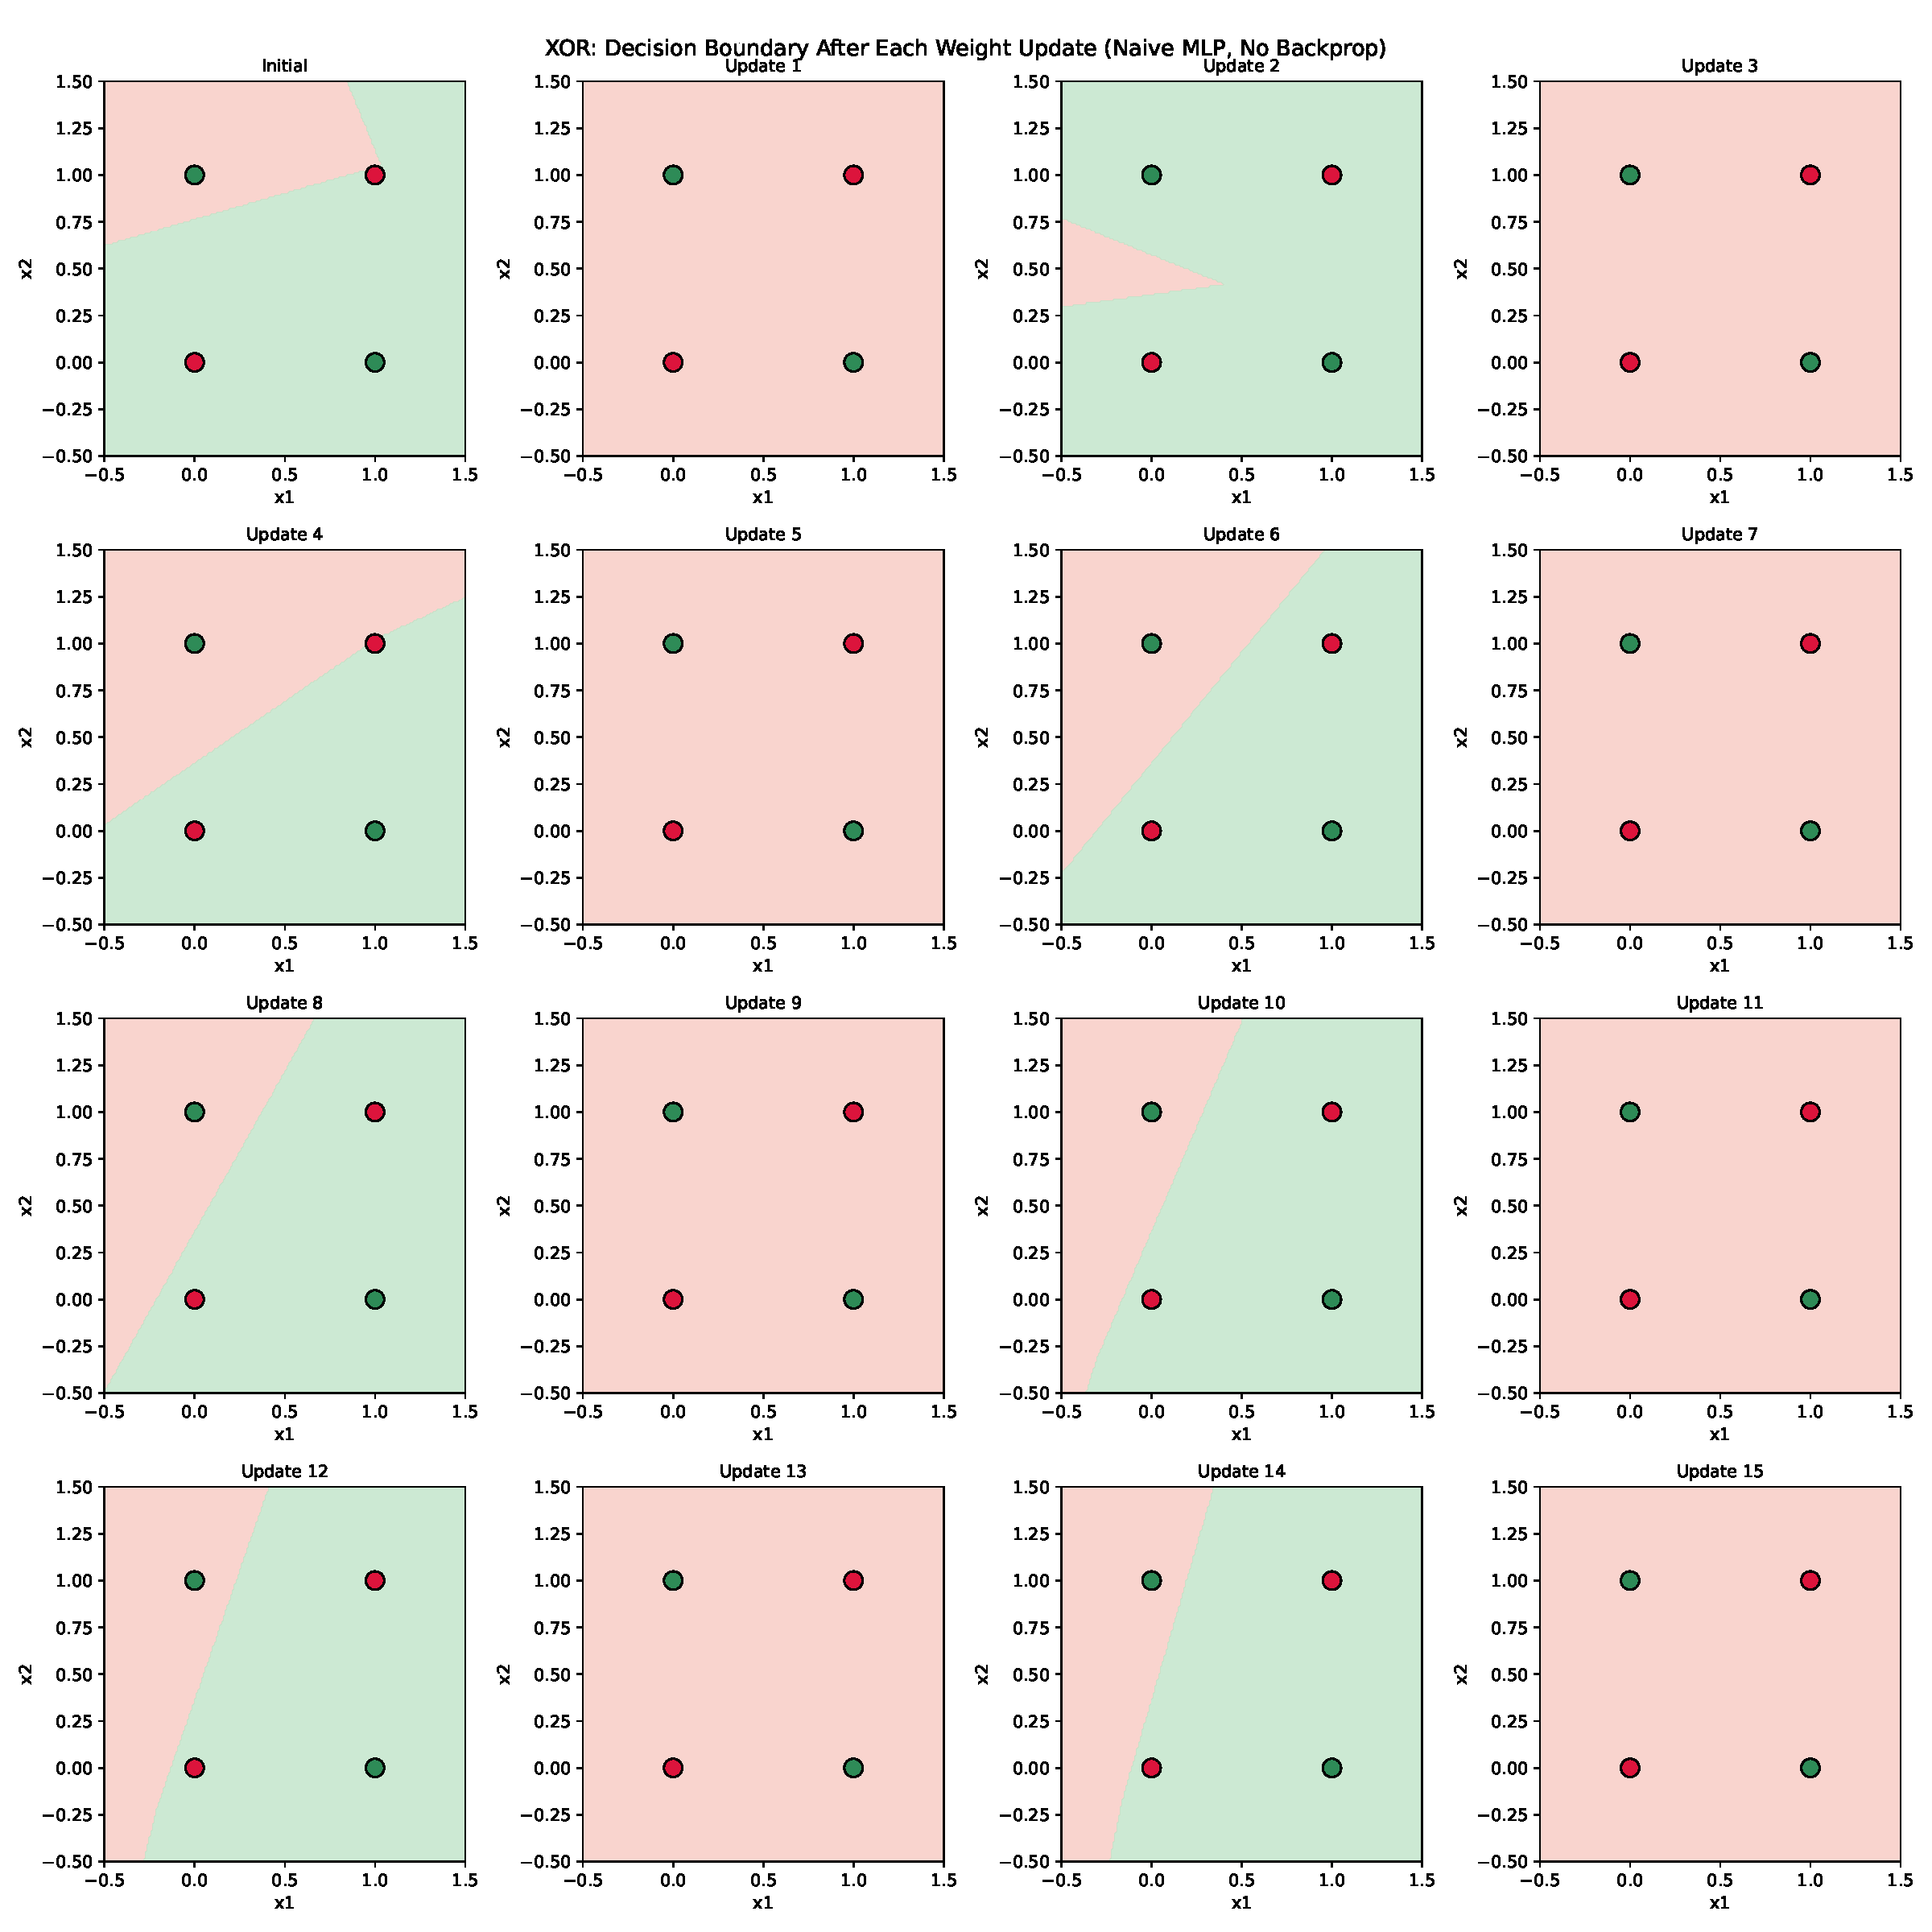
\includegraphics[width=0.95\textwidth]{xor_mlp_decision_boundaries.pdf}
\caption{XOR: Decision Boundary After Each Weight Update (Naive Multi-Layer Perceptron, No
Backpropagation).}
\end{figure}

\begin{figure}[h!]
\centering
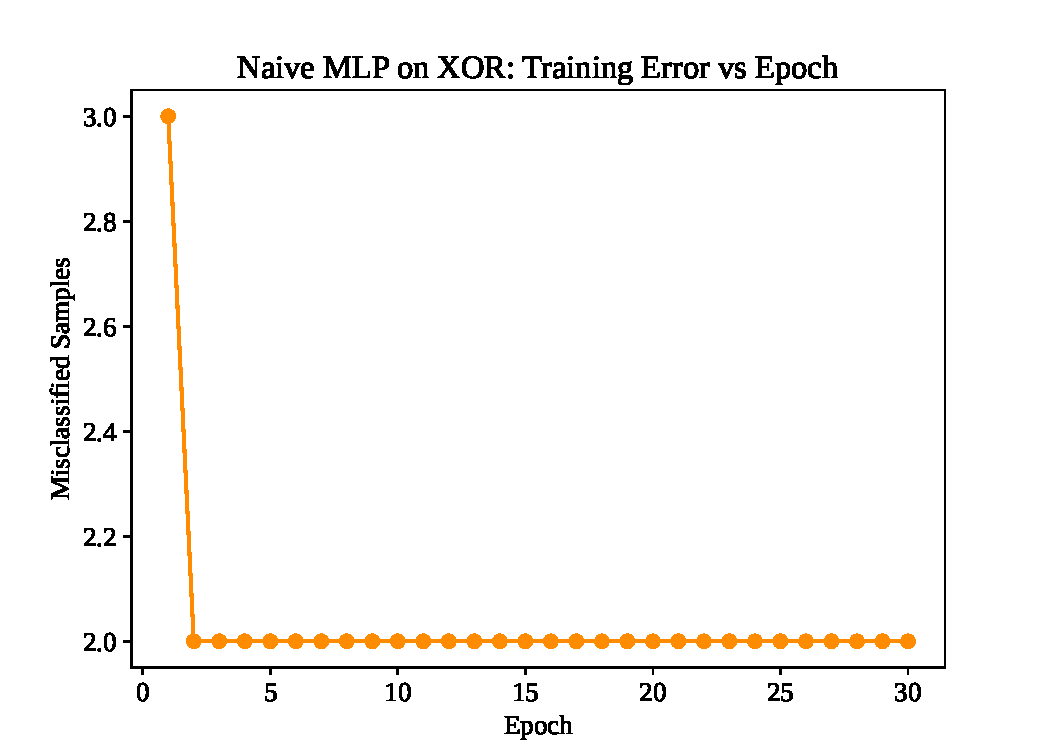
\includegraphics[width=0.65\textwidth]{xor_mlp_error_vs_epoch.pdf}
\caption{Naive Multi-Layer Perceptron on XOR: Training Error vs Epoch.}
\end{figure}

\section*{Analysis: The Pattern That Prevents Convergence}
The error count drops from 3 to 2 misclassified samples after the first epoch and then gets stuck
at exactly 2 for all the remaining 29 epochs. The network never reaches 0 errors.

Looking at the weight log, the same two samples, $(0,1)$ and $(1,1)$, are misclassified in every
epoch after the first. Each time, the hidden and output weights are updated in the same direction
as before, so the hidden layer weights keep growing in size (for example the first hidden weight
goes from about $-0.03$ after epoch 1 to about $-3.0$ by epoch 30), but the output weights,
$W_{out}$, stop changing completely after epoch 2 and stay fixed at $[-0.188, -0.027]$.

This happens because of how the naive rule updates the hidden layer. The hidden neurons use a
step activation, so their output is only ever 0 or 1, no matter how large the hidden weights get.
Once the sign of the hidden neuron's weighted sum stops flipping for a given input, that hidden
neuron's activation for that input is frozen, even though the raw weight values keep climbing.
Since the output weights only ever see 0s and 1s coming out of the hidden layer, once the hidden
activations settle into a fixed pattern for the two problem inputs, the output neuron's decision
for those two inputs is frozen too. From that point on, every update just makes the weights bigger
in the same direction without ever flipping any sign, so the same 2 samples stay wrong forever.

The deeper reason this happens is that the naive rule updates every hidden neuron using the same
output error, with no way to tell each hidden neuron how much it personally contributed to that
error. A proper multi-layer network needs backpropagation, which uses the chain rule to work out a
separate error term for each hidden neuron based on the output weight connected to it and the
derivative of its own activation function. Step activation has a derivative of 0 almost everywhere,
so even if backpropagation were applied here, no gradient could flow back through it. This is the
same limitation discussed earlier in this report for Step vs Sigmoid: without a differentiable
activation and a proper backpropagated error term for each hidden neuron, a multi-layer network has
no way to learn a hidden representation that actually helps solve a non-linearly separable problem
like XOR, so training gets stuck at a fixed, incorrect solution instead of converging.

\end{document}
